\chapter{Running the PR2}
Running the PR2 requires a basic understanding of ROS (\href{http://www.ros.org}{http://www.ros.org}), the BSD-licensed Robot Operating System.  A ROS system consists of multiple processes running on multiple computers.  If you are not familiar with ROS, it is highly recommended that you follow some of the \href{http://www.ros.org/wiki/ROS/Tutorials}{beginner tutorials} on ros.org, since familiarity with ros tools will make using the robot much easier.  In particular, you should understand what a launch file is and how to run it, and how to run ROS with nodes on multiple computers. This chapter will walk you through starting up and running a PR2, using ROS.


\section{Getting set up}
\subsection{Out of the box}
If you are starting your PR2 for the first time at your institution, please read the previous sections,\ref{Setting up PR2 in your lab}.  This will give you advice on setting up the network, setting the administrative password, and picking a safe location for charging the PR2.  This chapter assumes that the PR2 is already set up for your lab.
\subsection{Batteries and power}
Before running the robot, you need to make sure it has power.  The battery life of the PR2 is approximately two hours, so keeping it plugged in when not in use is a good idea.  You can follow the instructions in this chapter to start up the PR2 while it is plugged into the power outlet, which will keep the batteries charged.
\subsection{Run-stop}
The PR2 will not run its motors unless both run-stop buttons (the red push-button on the middle of the PR2's back, and the yellow wireless run-stop transmitter) are enabled.  Before you operate the PR2, you should have the wireless run-stop nearby, so that you can shut down the motors if you need to.  Before turning on the robot, press the red button on the wireless run-stop transmitter to prevent the motors from moving before you are ready.

%Add image of red push-button on PR2's back here
\begin{figure}[h]
\centering
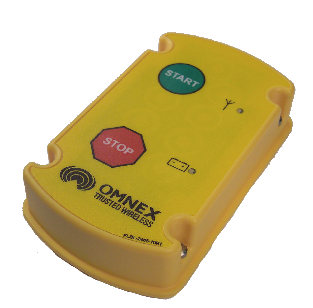
\includegraphics[width=150px]{run_stop.png}
\caption{The PR2 wireless run-stop.}
\label{fig:runstop}
\end{figure}

\subsection{Getting an account}
Before using the PR2, you will also need an account on the robot computers.  If you try to log in to the robot and the robot administrator has not created an account for you on the robot yet, then you will see, ``Permission denied, please try again'' when you try to log in to the robot. Ask the robot administrator to create an account for you, using the instructions in section \ref{creating accounts}.
\section{Turning PR2 on}
To turn the PR2 on, you should first verify that the wireless run-stop is off. On the wireless run-stop, press the red button, and make sure there are no flashing lights on the wireless run-stop. Then switch the red DC breaker on the back panel of the robot to the ``on'' position.  

\begin{figure}[h]
\centering
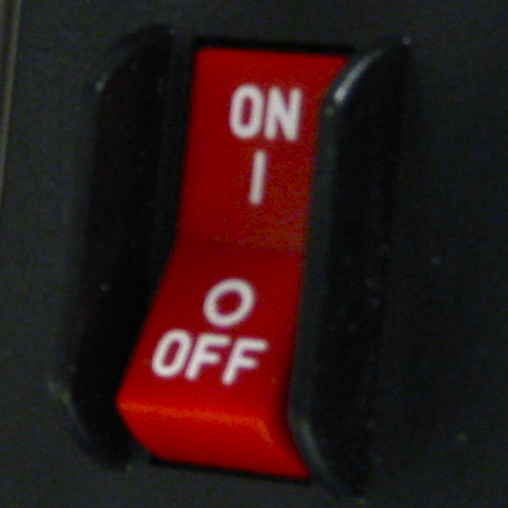
\includegraphics[width=50px]{dc_breaker.png}
\caption{The PR2 DC breaker switch in the ON position.}
\label{fig:dc_breaker}
\end{figure}

You should see the red lights on the computers turn on, hear the fans spin up, and hear several beeps from the computers as they boot.  The process of booting the computers will take about 5 minutes.  If the robot is already running, you can skip this step (but should still disable the wireless run-stop).
\subsection{Logging in}
Once the robot is on, \href{http://unixhelp.ed.ac.uk/CGI/man-cgi?ssh}{ssh} into the main computer using the account created for you by the administrator. 

In the following tutorial, we will use pr\textcolor{red}{x}1 to refer to the first computer on robot \textcolor{red}{x}.  Ask your robot  administrator what name you should use for the robot you want to run. To log in to the robot, type
\begin{verbatim}
ssh username@prx1
\end{verbatim}
You will notice that you are already set up with a ROS environment.  To see what packages are available to you, type
\begin{verbatim}
rospack list-names
\end{verbatim}
and you should see a list of the ros packages currently on your path.
%LT: What if they don't see this? What should they do? Contact administrator and say X?

\subsection{Checking for other users}
If you logged in to a robot that was already running, you should check to see if anyone else is using the robot.  To find out who else is using the robot, type
\begin{verbatim}
ckill list
\end{verbatim}
This will show you what programs are currently running on the robot.  If other people have processes running on the robot, you will need to find out if you can interrupt their work. You should find out who is on the robot and ask them to allow you to kill their processes so that you can work on the robot.  If you cannot find the people running processes on the robot, ask the robot adminstrator for guidance on what the policy is in your lab. If it is fine for you to kill the other processes running on the robot, you can type
\begin{verbatim}
sudo ckill kill
\end{verbatim}
and all the processes that are being run on the robot will be killed.
\section{Starting the software}
The launch file /etc/pr2/pr2.launch is used to start up the basic functionality of the robot.  This includes drivers for the sensors, motors, speakers, projector, power system, and joystick as well as the default set of realtime controllers, processing and logging of diagnostics information, and monitors for various types of problems your robot could experience.  On a new robot, this launch file is standard, but if the robot you are working on has been altered (e.g., has additional sensors, has only one arm), then it is likely that someone administering the robot has also updated the /etc/pr2/pr2.launch file to work with your robot's configuration.

Once you are logged in and ready to start the robot, you can run the robot by typing
\begin{verbatim}
pr2 start
\end{verbatim}
OR
\begin{verbatim}
roslaunch /etc/pr2/pr2.launch
\end{verbatim}
to start up the pr2.  Running pr2 start will start the roslaunch for you in the background as a system user. This will allow you to continue to use your current terminal and the robot will keep running after you log out.  

If you prefer to see everything that is going on, you can run the roslaunch manually, but you will need to keep that window open until you are done using the robot. Closing that the terminal in which you roslaunched will %LT: How would you describe what happens if you closed or ctrl-C'ed that terminal?
.

The robot should now be running, but since you have the wireless run-stop disabled, the motors will not be moving.  

If you used ``pr2 start'' then you will not need to open a new terminal to complete other commands. You can type 
\begin{verbatim}
rostopic list
\end{verbatim}
to see the topics being published by the system. 

If you used ``roslaunch'' to start the robot, then you will need to open a new terminal and type
\begin{verbatim}
ssh username@prx1
rostopic list
\end{verbatim}
to see what topics are being published by the system in the new terminal while the roslaunch continues to run in the original terminal.

\section{Running the dashboard}
When running the robot, the pr2\_dashboard should always be up on your screen.  This is how the robot software will let you know if something is going wrong, and is also how you turn the motors and power on and off.  On a computer with a built ROS installation (e.g., the base-station desktop computer that ships with the robot), set your ROS\_MASTER\_URI to point at the master running on the robot and launch the dashboard by typing
\begin{verbatim}
export ROS_MASTER_URI=http://prx1:11311
rosrun pr2_dashboard pr2_dashboard
\end{verbatim}
You should see the pr2\_dashboard control panel (a graphical user interface) appear and provide you with information about the state of the robot.  Take a moment to review the state of the robot. You can get a sense for the health of your robot by looking at the diagnostics information; click on the wrench on the far left.  Since you have the run-stop disabled, you see that the motors are giving you a warning (CURRENTLY THIS IS AN ERROR.  SHOULD CHANGE TO WARNING BY ROBOT SHIP DATE).  You should see a warning because the robot was just turned on and the encoders on the joints have not been calibrated yet.
If you see warnings or errors in any other sections, you should read the error messages and try to figure out what the problem is.  Ask your robot administrator for help if there are errors that you do not understand.
\subsection{Understanding pr2\_dashboard}
When running the PR2, the most important piece of software for you to understand and control the state of the system is the pr2\_dashboard.
pr2\_dashboard, Figure~\ref{fig:dashboard}, is a GUI for debugging and controlling low-level state of the PR2. The dashboard displays the diagnostic, 
circuit breaker, run-stop, and battery status.
\begin{figure}[h]
\centering
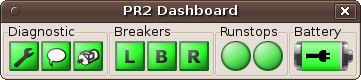
\includegraphics[scale=0.5]{pr2_dashboard.png}
\caption{The PR2 dasboard.}
\label{fig:dashboard}
\end{figure}
\begin{description}
\item[Diagnostic Status] The state of the robot is shown by the diagnoctic indicators in the pr2\_dashboard. \\

    \newcolumntype{S}{>{\centering\arraybackslash} m{.9cm} }%
    \begin{tabular}{m{6cm}SSSS}
    Component & OK & Warn & Error & Stale\\
    &&&&\\
    Diagnostics: Clicking pops up the Robot Monitor & 
\includegraphics[scale=0.5]{diag_ok.png}&
\includegraphics[scale=0.5]{diag_warn.png}&
                                                      
\includegraphics[scale=0.5]{diag_error.png}&
\includegraphics[scale=0.5]{diag_stale.png}\\
    &&&&\\
    Rosout: Clicking pops up rxconsole & 
\includegraphics[scale=0.5]{rosout_ok.png}&
\includegraphics[scale=0.5]{rosout_warn.png}&
                                        
\includegraphics[scale=0.5]{rosout_error.png}&
\includegraphics[scale=0.5]{rosout_stale.png}\\
    &&&&\\
    Motors: Clicking allows you to halt or reset motors & 
\includegraphics[scale=0.5]{motor_ok.png}& N/A &
                                                          
\includegraphics[scale=0.5]{motor_error.png}&
\includegraphics[scale=0.5]{motor_stale.png}\\
   \end{tabular}

\item[Circuit Breaker Status] The circuit breakers are labeled L/B/R, which stand for Left Arm, Base/Spine, and Right Arm. 
Each breaker can be in one of four states, and clicking on any of the breakers will pop up a menu (Figure~\ref{fig:breaker_menu}), allowing you to change the state of one or all of them:
\begin{figure}[h]
\centering
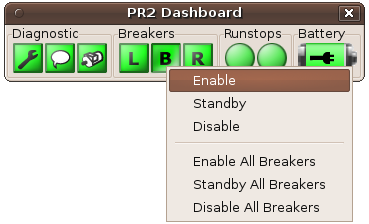
\includegraphics[scale=0.5]{breakers_menu.png}
\caption{The circuit breaker options menu.}
\label{fig:breaker_menu}
\end{figure}

    \newcolumntype{S}{>{\centering\arraybackslash} m{1.7cm} }%       
    \begin{tabular}{m{2.6cm}SSSS}
     & Enabled & Standby & Disabled & Stale\\
    Breaker Status & 
\includegraphics[scale=0.5]{L_ok.png}
\includegraphics[scale=0.5]{B_ok.png}
\includegraphics[scale=0.5]{R_ok.png}&
                     
\includegraphics[scale=0.5]{L_stby.png}
\includegraphics[scale=0.5]{B_stby.png}
\includegraphics[scale=0.5]{R_stby.png}&
                     
\includegraphics[scale=0.5]{L_dis.png}
\includegraphics[scale=0.5]{B_dis.png}
\includegraphics[scale=0.5]{R_dis.png}&
                     
\includegraphics[scale=0.5]{L_stale.png}
\includegraphics[scale=0.5]{B_stale.png}
\includegraphics[scale=0.5]{R_stale.png}\\
   \end{tabular}



\item[Runstop Status] The runstop indicators display the staus of the PR2 runstops and their states cannot be changed using the dashboard. 
There are two run-stops on the robot, a wireless run-stop, see \ref{wirelessrunstop}, and a red push button run-stop on the back of the robot.\\

    \newcolumntype{S}{>{\centering\arraybackslash} m{2.5cm} }%                                                                                                         
    \begin{tabular}{m{2.6cm}SSS}
     & OK & Physical Stop & Wireless Stop\\
    Runstop Status & 
\includegraphics[scale=0.5]{runstop-green.png}
\includegraphics[scale=0.5]{runstop-green.png}&
                     
\includegraphics[scale=0.5]{runstop-red.png}
\includegraphics[scale=0.5]{runstop-green.png}&
                     
\includegraphics[scale=0.5]{runstop-yellow.png}
\includegraphics[scale=0.5]{runstop-red.png}\\
   \end{tabular}


\item[Battery Status]
%LT: NEED CONTENT HERE; how should one interpret the battery status indicator?
\end{description}

\section{Calibrating the joints}
If you do not discover any problems in the diagnostics, and you want to continue with robot bringup, press the green button on the wireless run-stop.  This should change the state of the run-stop indicator on the dashboard to a green circle, and will allow the robot to turn power on for the motors.  The next step is to enable the circuit breakers (marked L, B, R).  When you click on the circuit-breaker icon, select ``enable all'' from the menu to turn on all three breakers.

Finally, check that the area around the robot is safe for it to move its arms, click on the picture of a motor, and select ``reset motors.''  When you do this, the robot will move its joints to find the absolute reference positions of each joint so that it can calibrate the mechanism.  When calibration is finished, you should see all the icons in the dashboard reading OK.
\section{Driving with the joystick}
To move the robot, you can now drive it around with the joystick.  To do this, you will need to open a new ssh connection to the robot and run the teleop\_joystick launch file
\begin{verbatim}
ssh username@prx1
roslaunch pr2_alpha teleop_joystick.launch 
\end{verbatim}
(NOTE- Move out of pr2\_alpha before release and document button mapping)
Once the teleop\_joystick node is running, press the parring button (Figure~\ref{fig:pairing}) in the middle of the joystick to pair it with the robot (the four LEDs on the jostick will flash when paired). Then you should be able to drive the robot around.
\begin{figure}[H]
\centering
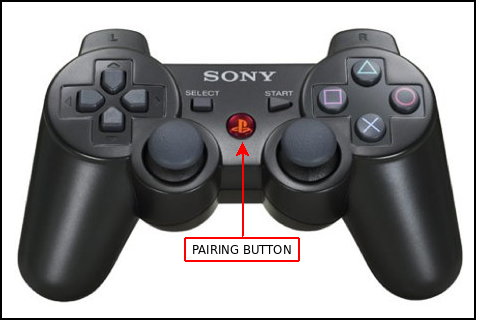
\includegraphics[scale=0.40]{pairing.png}
\caption{Pairing the joystick with the PR2.}
\label{fig:pairing}
\end{figure}
For more information about how to drive the robot around, see the 
\href{http://www.ros.org/wiki/ps3joy/Tutorials/UsingJoystickWithPR2}{ps3joy} tutorial at \href{http://www.ros.org}{ros.org}. 

\section{Visualizing sensor data}
To see the sensor data from the robot, you can use rviz on the offboard computer (e.g., base station).  Again, you will need to configure the ROS\_MASTER\_URI to point at the robot, so run
\begin{verbatim}
export ROS_MASTER_URI=http://prx1:11311
rosrun rviz rviz
\end{verbatim}
and you should see rviz launch with a visualization of the robot.  For more information about how to view different types of data coming from the robot, See the \href{http://ros.org/wiki/rviz}{rviz} documentation at \href{http://www.ros.org}{ros.org}.
(TODO - WITH THE CURRENT LAUNCH FILE, YOU WILL NOT BE ABLE TO SEE CAMERA DATA)

\section{What next?}
From here, you can do what you want on the robot.  Point to instructions for writing code and to a list of other applications and things to do with the robot.
